\section{Typical designs of Tangible User Interfaces}

\begin{center}
\begin{table*}[ht]
\small
\hfill{}
\begin{tabular}[ct]{|p{3 cm}|p{4 cm}|p{4.5 cm}|p{4.5 cm}|}
 \hline
 Example  & Application Area & Hardware Characteristics & Special Characteristics \\
 \hline
 \hline
 metaDESK & Geographical Application & backprojected display \newline active and passive lens \newline assortment of physical objects \newline optical, mechanical and electromagnetic field sensors & collaborative \newline interaction on and above display\\
 \hline
 Tangible Views & Information Visualization & lightweight displays with infrared reflecting markers \newline tabletop surface \newline infrared cameras \newline top projector & Tangible Views not restricted in size or shape \\
 \hline
 Interactive Textbook & Additional contents to textbooks & desk \newline CCD camera \newline pan-tilt camera \newline video projector & matrix codes \newline template matching \newline finger gesture recognition \\
 \hline
 Tangible Query Interfaces & Large databases & display surface \newline query rack \newline query pads \newline parameter wheels \newline parameter bars \newline top projector & tokens representing expressions instead of individual information \newline RFID tags \newline tokens+constraints \\
 \hline
 The reacTable & Musical instrument & round table \newline infrared camera \newline pucks \newline projector under table \newline & pucks represent modular synthesizer component \newline finger gesture recognition \newline every information displayed is strictly relevant and informational \newline collaborative\\
 \hline
 Urp & urban planning & ordinary table \newline projectors \newline architectral models \newline additional tools & I/O Bulb infrastructure \newline accurate shadow casting \newline flow visualization \newline glimpser-and-voodoo \\
 \hline
\end{tabular}
\hfill{}
\caption{Design Examples of Tangible User Interfaces}
\label{tb:design}
\end{table*}
\end{center}


%http://www.guillaumeriviere.name/collection/tabletop.html
\begin{figure*}
\centering
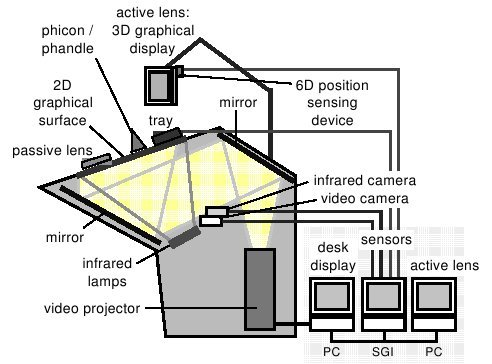
\includegraphics[width=0.7\textwidth]{figures/metaDeskHardware.jpg}
\caption{metaDESK Hardware Overview www.guillaumeriviere.name/collection/tabletop.html}
\label{fig:metadeskhardware}
\end{figure*}

In this section we will discuss different hardware implementations as well as software elements of tangible user interfaces and take a look on the different design spaces they are used in. 
% The interpretation of tangible user interfaces varies throughout the field. Ullmer and Ishii \cite{ullmer97} 

The possible applicatons TUIs can be used in depend highly on the application area. Not every TUI is suitable for every task. Therefore we first take a look at what areas can profit from using TUIs. 

Shaer and Hornecker \cite{hornecker10} give the following list of possible application domains:
\begin{itemize}
\item TUIs for Learning
\item Problem Solving and Planning
\item Information Visualization
\item Tangible Programming
\item Entertainment, Play, and Edutainment
\item Music and Performance
\item Social Communication 
\item Tangible Reminders and Tags
\end{itemize}

As this list already suggests, there are many areas in which a TUI can be used. But the specific design for each of these areas varies significantly. Therefore in this section we will take a look at different examples of TUIs used in different application areas to see in which way they differ. 

To accomplish this we will use the following examples: the metaDESK by Ullmer and Ishii \cite{ullmer97}, Tangible Views by Spindler, Tominski, Schuhmann and Dachselt \cite{spindler10}, Interactive Textbook by Koike, Sato, Kobayashi Y., Tobita and Kobayashi M. \cite{koike00}, Tangible Query Interfaces by Ullmer, Ishii and Jacob \cite{ullmer03}, the reacTable by Jord\`{a}, Geiger, Alonso and Kaltenbrunner \cite{jorda07} and Urp by Underkoffler and Ishii \cite{underkoffler99}. 

To gain a general overview of the mentioned examples we provide a table \ref{tb:design} giving in short detail the example with the specific application area, hardware features and special characteristics. 

What most of the TUIs have in common is the use of a projector to enhance the surrounding environment with information. But in terms of interaction they vary quite a bit. Some TUIs like the metaDESK system or the Tangible Query Interfaces rely solely on using physical objects for interaction, while other systems like the Interactive Textbook or the reacTable also take interaction using your finger and hand gestures into account.  

Now we will take a closer look at each of these systems. 






%http://www.guillaumeriviere.name/collection/tabletop.html
\begin{figure}
\centering
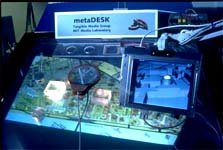
\includegraphics[width=0.45\textwidth]{figures/metaDesk.jpg}
\caption{metaDESK www.guillaumeriviere.name/collection/tabletop.html}
\label{fig:metadesk}
\end{figure}

\subsection{metaDESK}
One of the attemps in broadening the input possibilities to different devices is the metaDESK system introduced by Ullmer and Ishii \cite{ullmer97}. They describe a "Tangible User Interface" (TUI) as "a user interface employing physical objects, instruments, surfaces, and spaces as physical interfaces to digital information". 

The metaDESK system consists of: a desk, an active lens, one or more passive lenses, and an assortment of physical objects and instruments which are used on the desk's surface. 

The desk is build as a nearly-horizontal backprojected graphical surface and shows a general overview. 

The active lens is an arm-mounted flat-pannel display, allowing to navigate through the space above the tabletop surface. This allows a seamless interaction with three spaces at once: the physical space of the object, the 2D graphical space of the desk's surface and the 3D graphical space of the active lens.

The passive lenses are made out of an optically transparent surface and can be placed on the tabletop surface. They function as independent displays when augmented by the back-projected desk. It is also possible to place more than one lens on the tabletop surface and use them simultaneously without the need of additional active display resources.

The physical objects and instruments are tangible objects, real physical objects which can be touched and grasped. The models are taken from everyday objects from home, scientific instruments or drawing and design tools. The material they used was transparent machined acrylic, designed to minimize occlusion of the desk surface.

The components are sensed by an array of optical, mechanical and electromagnetic field sensors. An image of such a setup can be seen in Figure \ref{fig:metadesk} and an outline of the hardware positioning in Figure \ref{fig:metadeskhardware}.




The focus lies on the use of real physical objects as driving elements of human-computer interaction. The approach of Ullmer and Ishii tries to take elements of the GUI and bringing it into the real world as well as pushing forward from the unaugmented physical world, inheriting from vaious historical instruments and devices often "obsoleted" by the advent of the computer, like the active lens which is based on a jeweler's magnifying lens. 

The GUI icons are instantiated as "phicons" (physical icons), menus and handles are instantiated as TUI "trays" and "phandles" (physical handles), scales and scrollbars as TUI instruments such as a rotation constraint instrument. 

To test the system they implemented a prototype application called "Tangible Geospace" allowing interaction with geographical space.
The models themselves act as information containers about the object they represent as well as physical handles for manipulating the map.

The arm mounted active lens is coupled to the models and displays three-dimensional views of the scene and moving the lens makes it possible to navigate through 3D space. 

It is also possible to place a second object on the table, allowing the user to scale or rotate the map by moving the objects with respect to each other. This also allows collaboration as each object may be manipulated by an individual user. The sensing is performed by a computer-vision system inside the desk unit, along with magnetic-field position sensors and electrical contact sensors.

As alternative to the two phicon scaling/rotation interaction, a rotation constraint instrument made of two cylinders mechanically coupled by a sliding bar might be used.
Albeit the extension of input methods it is not the goal of metaDESK to replace GUIs, but rather to complement them by providing new opportunities for human-computer interaction. 

% personal idea
The original Paper was published in 1997 and so some parts of the hardware could be replaced with more recent advances in technology. For example for the active lens a modern tablet could be used. 




\subsection{Tangible Views}
Spindler, Tominski, Schuhmann and Dachselt \cite{spindler10} introduce 'tangible views' for use in Information Visualization as spatially aware lightweight displays that can be interacted with by moving them through the physical space on or above a tabletop surface. They wanted to create a seamless integration of interaction and display devices and new ways of visualizing and directly interacting with information. 

The motivation for their project is the difficulty of encoding all information in a single image once a data set exceeds a certain size or complexity. This problem can be solved spatially by providing multiple views on the data or embedding additional local views in the visualization or it can be solved temporally by changing the representations over time.

A Tangible View is a physical lightweight surface that users can hold in their hands. This surface is not restricted in size or shape and can for example be made out of regular cardboard. 

A setup for Tangible Views consists of a tabletop display, several infrared (IR) cameras and a top projector on the ceiling. To track the Tangible Views in space, small unobtrusive IR reflecting markers are placed at the corners or borders of the Tangible View. OpenGL is then used to emulate the physical space above the tabletop. This makes this lightweigth surfaces spatially aware as they are moved through the physical 3-dimensional space above the display surface. The tracking of the movement makes six degrees of freedom available: position (x, y, z) with respect to the interaction space and local orientation of the tangible view ($\alpha$, $\beta$, $\gamma$).
\begin{figure}
\centering
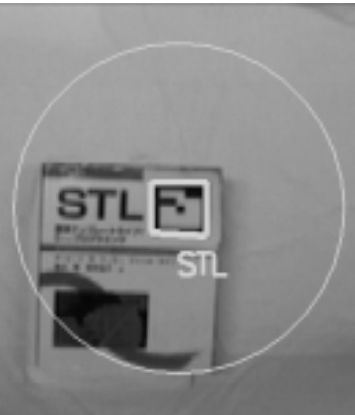
\includegraphics[width=0.45\textwidth]{figures/InteractiveTextbook4.jpg}
\caption{Automated recognition of a matrix code on a textbook page.}
\label{fig:textbook}
\end{figure}

Tangible views serve two purposes: It is used as a local display in conjunction with a tabletop display, and as an input device.
Using the top projector the specific graphical information is projected onto the tangible view.

It is also possible to use multiple tangible views at the same time. 
Tangible views do not exist on their own, but are integrated into an environment of one or more stationary displays of arbitrary size, shape and orientation. 
They also describe a basic display configuration consisting of a horizontal tabletop for the main context view and tangible views as local views into the information space. This relates to the focus and context concept.

In summary tangible views:
\begin{itemize}
\item Integrate display an interaction device.
\item Enhance common 2D interaction with additional 3D interaction
\item Replace virtual views by physical, tangible views.
\end{itemize}

As Tangible Views play an important role in Information Visualization we will treat this subject in section four in more detail.

\begin{figure}
\centering
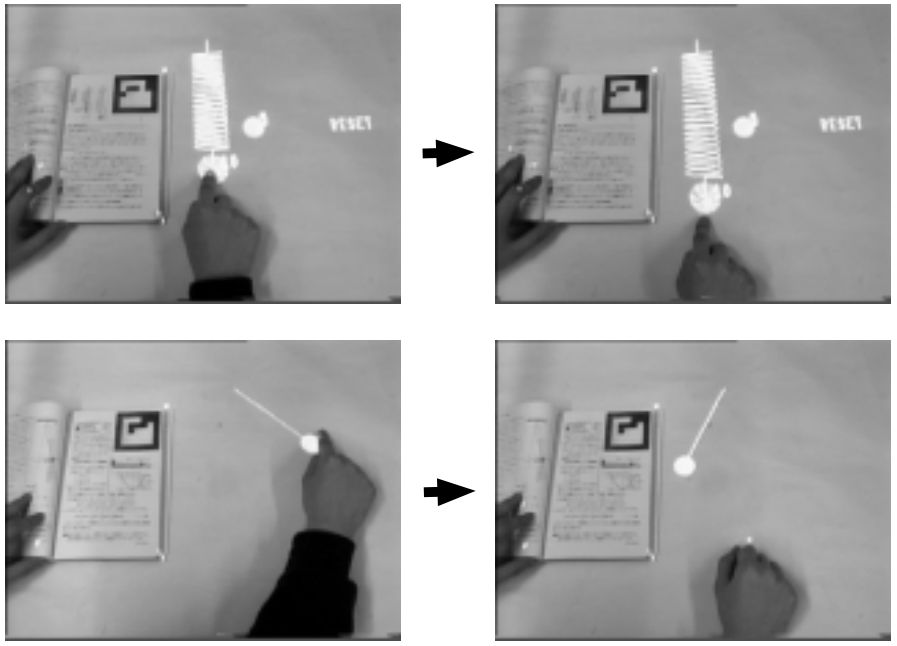
\includegraphics[width=0.45\textwidth]{figures/InteractiveTextbook.jpg}
\caption{Interaction with additional content.}
\label{fig:textbook2}
\end{figure}

\subsection{Interactive Textbook}

Koike, Sato, Kobayashi Y., Tobita and Kobayashi M. \cite{koike00} implemented two interface prototypes for the augmented desk interface system EnhancedDesk. 

The goal of their work was to provide additional interactive contents and to enable a more natural interaction. 


The system itself consists of a desk, a CCD camera and a pan-tilt camera, and a video projector. 
The pages in the textbook that have extra content available are marked with a matrix code as can be seen in Figure \ref{fig:textbook}. 

When the user pages through the textbook, the camera scans the pages and, if a matrix is present, identifies the unique ID of the matrix code as well as its size and orientation. According to this information the system then decides where to project the digital contents. This ensures that the information is always placed where the information is needed and in the correct slant. 

The automatic retrieval using the matrix code is only one part of the system. The second is enabling dynamic manipulation by recognition of finger gestures. 

To allow for recognition of gestures, the infrared camera and template matching is used. The temerature range for the infrared camera threshold is set to approximately human body temperature. The reason behind the infrared camera is that a normal camera would fail to find human skin regions. Thats because the LCD projector projects vaious kinds of objects like text or figures onto the human skin which alters the color of the human skin completely. Also the background changes dynamically. 

With template matching the palm center and fingers are recognized. This allows for interaction with the projected objects as can be seen in Figure \ref{fig:textbook2}. 




\subsection{Tangible Query Interfaces}

The Tangible Query Interfaces by Ullmer, Ishii and Jacob \cite{ullmer03} extends tangible interfaces. 
This approach allows the interaction with large aggregates of information which are stored in a database. 
Physically constrained tokens represent database parameters. These tokens can be used to express, manipulate and visualize parameterized database queries. As the number of physical tokens is limited, so is the number of information elements a TUI can practically be used to manipulate. 

Operations on individual elements in a large aggregate of information may be difficult. Therefore, instead of using the physical objects to represent individual information elements, the physical objects indirectly reference information by representing expressions (database parameters) that hold over large aggregates of information.

The Tangible Query Interface itself is build out of a display surface, a "query rack", "query pads", "query bars", parameter wheels and a projector. Figure \ref{fig:tanquery} shows such a setup.

"query racks" express queries composed of the corresponding parameters. 
By manipulating the physical tokens thresholds can be modified, boolean relationships expressed, and the visualization of the the query results can be controlled. 

The parameter wheels are small cylindrical tokens. They have RFID tag enbedded and are faced with cardstock labels. Parameter wheels represent fields of the database with continuous or discrete data. The associated value ranges remain persistently bound when moved to or from the "query rack". This eases the change of view. 

\begin{figure}
\centering
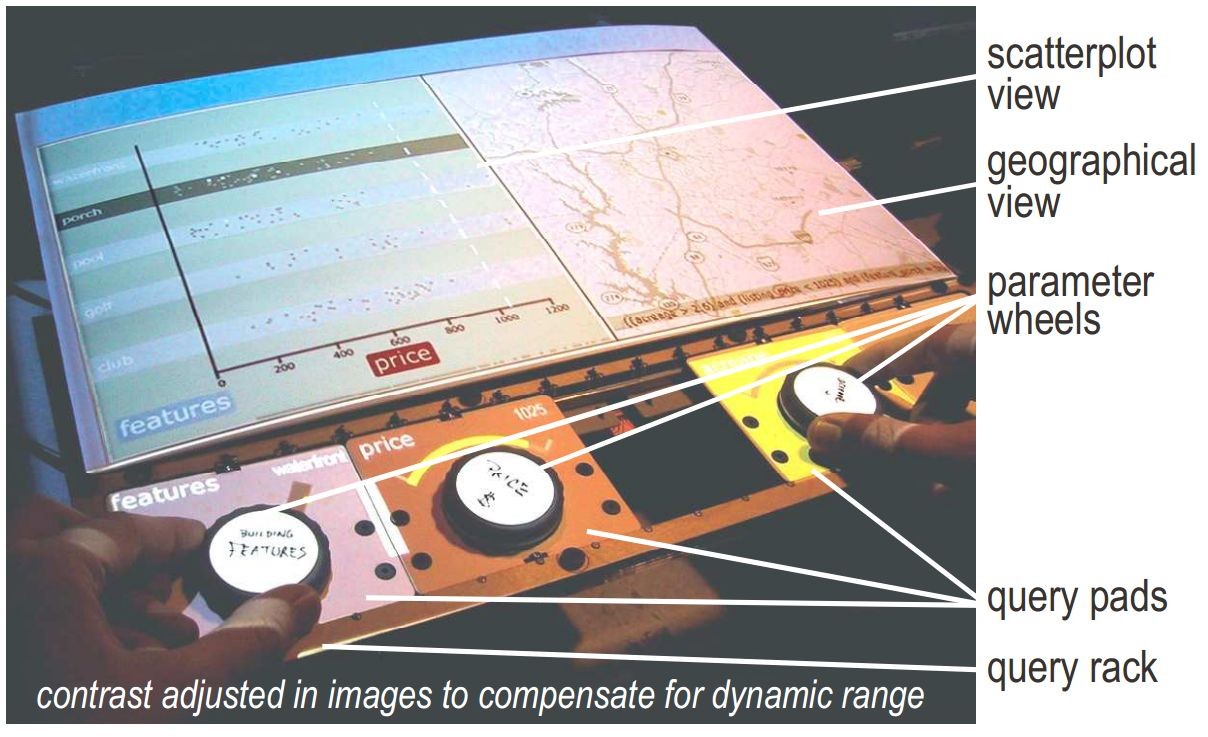
\includegraphics[width=0.45\textwidth]{figures/TangibleQueryInterfaces.jpg}
\caption{Tangible Query Interface}
\label{fig:tanquery}
\end{figure}

The "query rack" is made out of a series of "query pads" and each "query pad" has a receptacle for a parameter wheeel. When a wheel is placed on one of the pads the corresponding parameter is part of the active query. 

Besides the "query rack" they also made parameter bars as can be seen in Figure \ref{fig:tanquery2}. These bars have an avtice display embedded to indicate the identity of the active parameter and also show a histogram of the values. The parameter bars can be bound dynamically to new parameters by placing them near a binding point near a GUI monitor with their internal displays updating accordingly. On the parameter bar there are two sliders embedded allowing to modify both upper and lower bound of a target parameter range. 

The display surface is placed adjacent to the query rack. 
The projector illuminates both the display and the "query rack". 

Additionally the spacial placement of the pads decides how the associated parameters are used in the query. Spatially close pads indicate that the parameters are combined using an AND relationship. Spatially separated pads indicate an OR relationship. 

Tangible Query Interfaces follow the "tockens+constraints" approach where tokens are discrete, spatially reconfigurable physical objects representing digital information or operations. Constraints are confining regions within which tokens can be placed and the placement within the confines decides the digital operations or properties that are applied to the tokens. 

If a token is placed it is part of the actual query. The physical placement decides the view selection, the physical rotation decides the parameter value selection. When tokens are placed physically adjacent a boolean operation is performed. 

\begin{figure}
\centering
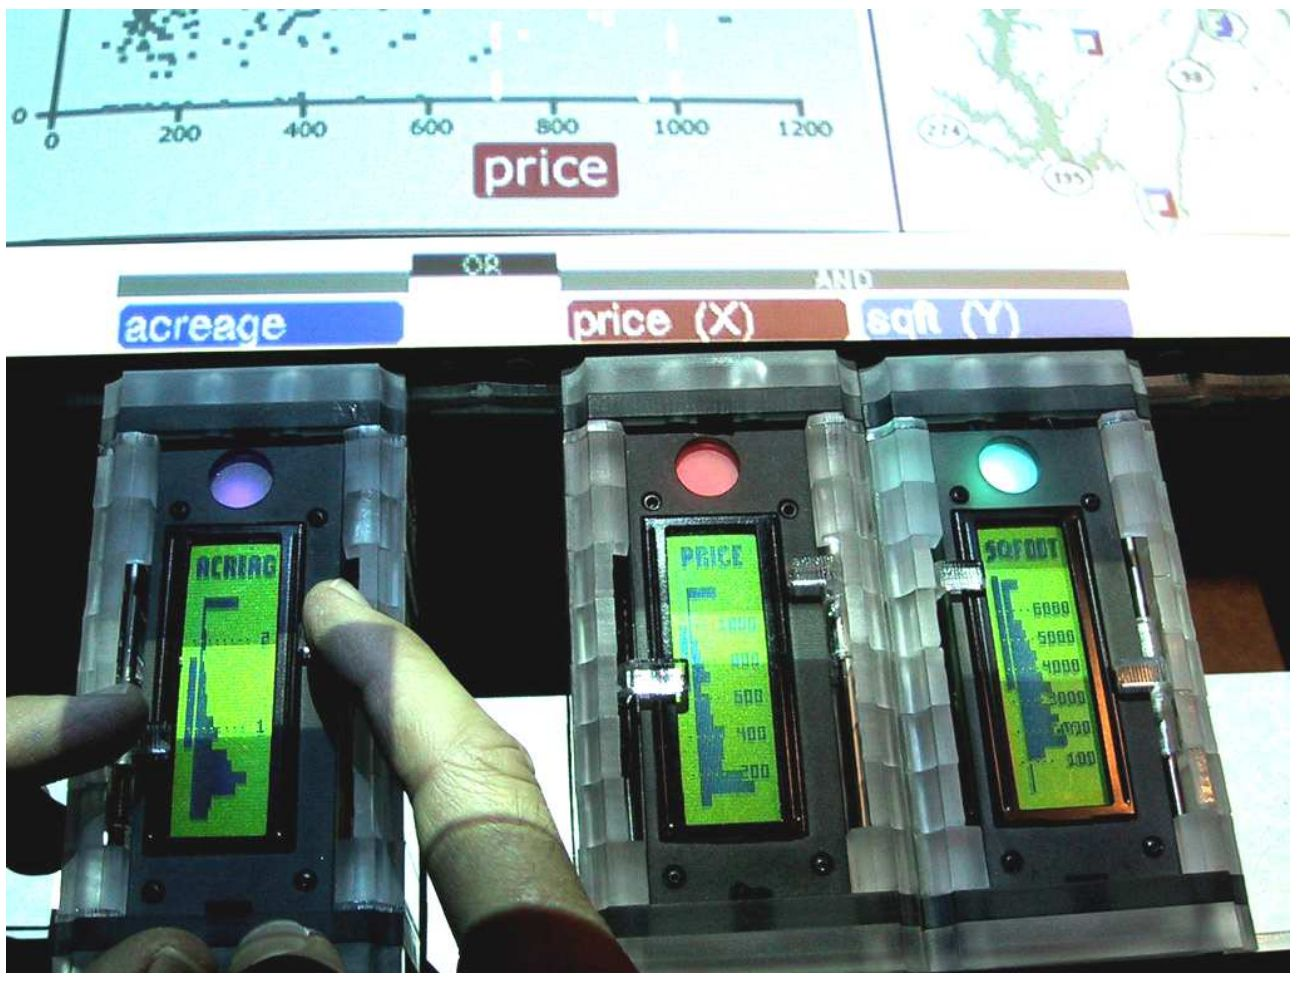
\includegraphics[width=0.45\textwidth]{figures/TangibleQueryInterfaces3.jpg}
\caption{Parameter bar}
\label{fig:tanquery2}
\end{figure}

\begin{figure*}
\centering
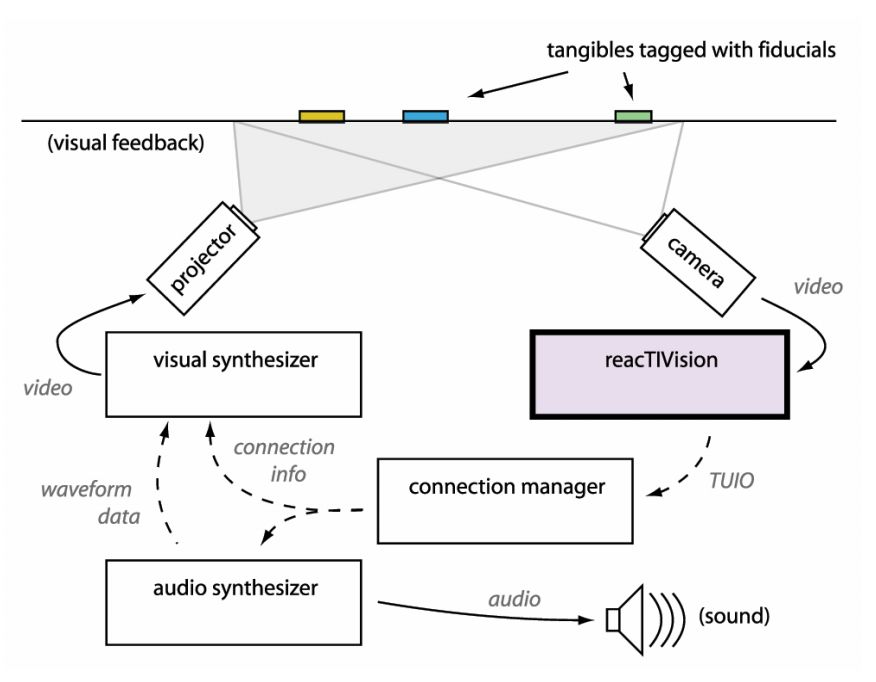
\includegraphics[width=0.7\textwidth]{figures/reactable-setup.jpg}
\caption{reacTable setup}
\label{fig:reactablea}
\end{figure*}

\subsection{The reacTable}

The reacTable is a musical instrument based on a tableop interface by Jord\`{a}, Geiger, Alonso and Kaltenbrunner \cite{jorda07}. "The reacTable seeks to combine immediate and intuitive access in a relaxed and immersive way, with the flexibility and the power of digital sound design algorithms, resulting in endless improvement possibilities and mastership" \cite{jorda07}. It's designed for installations, casual users and professionals in concerts. 

Digital musical instruments can be divided into a gestural controller or input device that takes the control information from the performers and a sound generator that plays the role of the excitation source. 

As a controller a simple computer mouse, computer keyboard or MIDI keyboard can be used, but using sensors and appropriate analogue to digital converters any control signal from the outside can be converted into control messages understandable by the digital system. 

The reacTable is based on a round table. This way it has no head position or leading voice and no privileged points-of-view or points-of-control. It uses a radial coordinate system and a radial symmetry. 
This enables several musicians to share the control of the instrument. 

Each reacTable object (puck) represents a modular synthesizer component and has a dedicated function for the generation, modification or control of sound. These objects are automatically connected and disconnected by a simple set of rules, according to their type, affinity and proximity with the other neighbours. The topologies are permanently presented on the table surface by a graphic synthesizer. The auras around the physical objects show information about their behaviour, their parameter values and configuration states. The lines connecting the objects show the real waveforms of the sound flow being produced or modified at each node. 



\begin{figure}
\centering
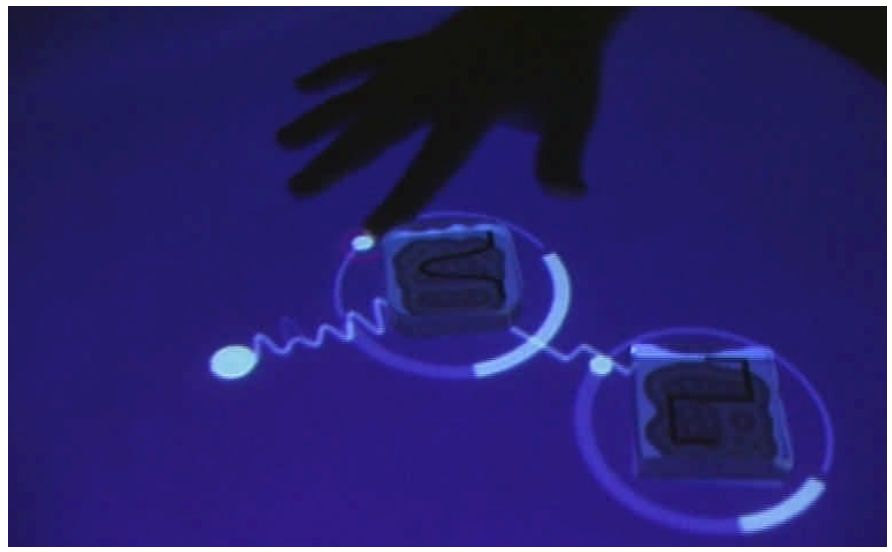
\includegraphics[width=0.45\textwidth]{figures/reactable2.jpg}
\caption{reacTable interaction example}
\label{fig:reactableb}
\end{figure}

Pucks and fingers are tracked by an IR camera placed beneath the translucent table and thus avoiding any type of occlusion. This setup can be seen in Figure \ref{fig:reactablea}.

They take use of Computer Vision (CV) techniques, taking advantage that CV can be combined with beneath projection, permitting a compact all-in-one system in which both camera and projector are hidden. Also the number of markers is almost unlimited (at the time the paper was written, several hundreds. 
Also the number of pucks is only limited by the table surface and it's possible to detect their orientation and not only their position. 
The use of CV also makes it possible to use cheap pucks, such as specially printed business cards. An example of merkers can be seen in Figure \ref{fig:reactable2}.

\begin{figure}
\centering
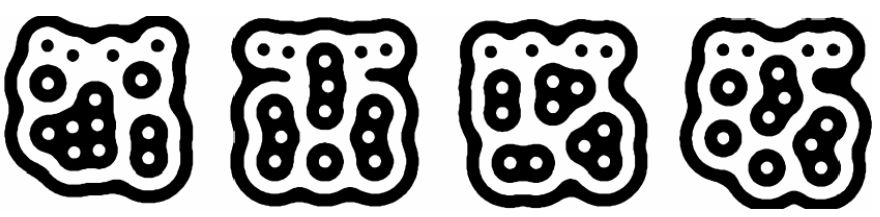
\includegraphics[width=0.45\textwidth]{figures/reactable-amoebamarkers.jpg}
\caption{reacTable markers from a reactTIVision set.}
\label{fig:reactable2}
\end{figure}

The reacTable uses it's own vision engine, the ReacTIVision. It is a high-performance computer vision framework for the fast and robust tracking of fiducial markers, specially designed graphical symbols allowing identification and location of physical objects, in a real-time video stream. This allows for low latency and high temporal resolution (~60 fps) needed for a real-time musical instrument. 
This makes it possible to create and manipulate data flows. 

All reacTable objects can be spun to control one of their internal parameters (like frequency or speed) and a second parameter is controlled by dragging the finger around the object's perimeter (like the amplitude) which can be seen in Figure \ref{fig:reactableb}.

The reacTable's objects can be categorized into six different functional groups: audio generators, audio filters, controllers, control filters, mixers and global objects (which influence the behaviour of all objects within the area of influence). Each familiy is associated with a different puck shape as can be seen in Figure \ref{fig:reactable3}.

On the visual display any shape, form line or animation drawn is strictly relevant and informational. 

\begin{figure}
\centering
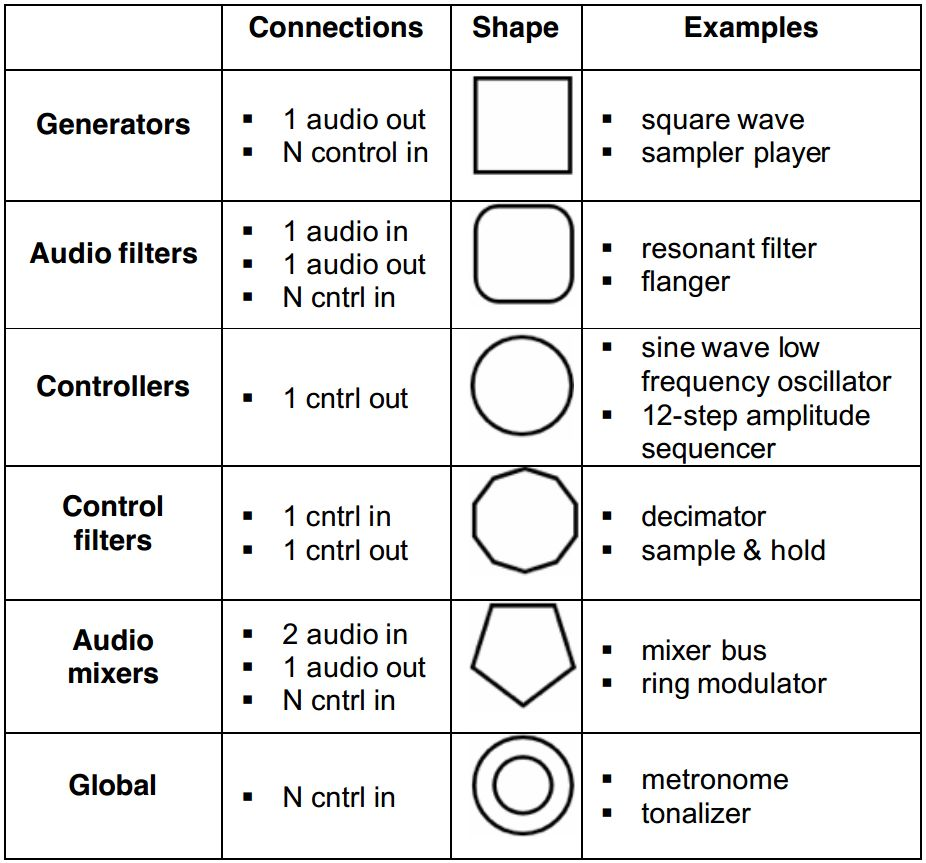
\includegraphics[width=0.45\textwidth]{figures/reactable-shapes.jpg}
\caption{reacTable object types}
\label{fig:reactable3}
\end{figure}


\subsection{Urp}

The \textit{Urp} is a system for urban planning developed by Underkoffler and Ishii \cite{underkoffler99} with the large scale scope of a wholesale transformation of architectural space to make of each surface an information-display-and-interaction structure. 
The constraints considered are: shadows, proximities, reflections, wind and visual space. 

The application is based around the \textit{I/O Bulb} infrastructure which allows physical architectural models placed on an ordinary table surface to cast accurate shadows for specific times of the day, as well as to reflect light off glass surfaces and affect a real-time and visually coincident simulation of pedestrian-level windflow. 
It uses light bulbs modified to be capable of projecting images into the space around it (in the work of Underkoffler and Ishii replaced by commercially available projectors). A tiny video camera looks out at the world around the bulb. 
This structure is capable of simultaneous input and output. 

\textit{Luminous Room} refers to a collection of many \textit{I/O Bulbs}, computationally interlinked and distributed throughout an interior architectural space. This aggregate addresses every portion of a room. 

\textit{Urp} employs the \textit{glimpser-and-voodoo} vision analysis pipeline \cite{underkoffler98} to identify and locate its component objects. The specific, known objects are optically tagged with small colored dots. The low-level machine vision system called \textit{glimpser} is used to find all colored dots. The list of dots is then passed to \textit{voodoo} with which it communicates through a client-server pair. 
\textit{voodoo} then tries to recognize as many known patterns as possible among each collection of dots. 
The patterns themselves are defined by \textit{Urp}. 

\begin{figure}
\centering
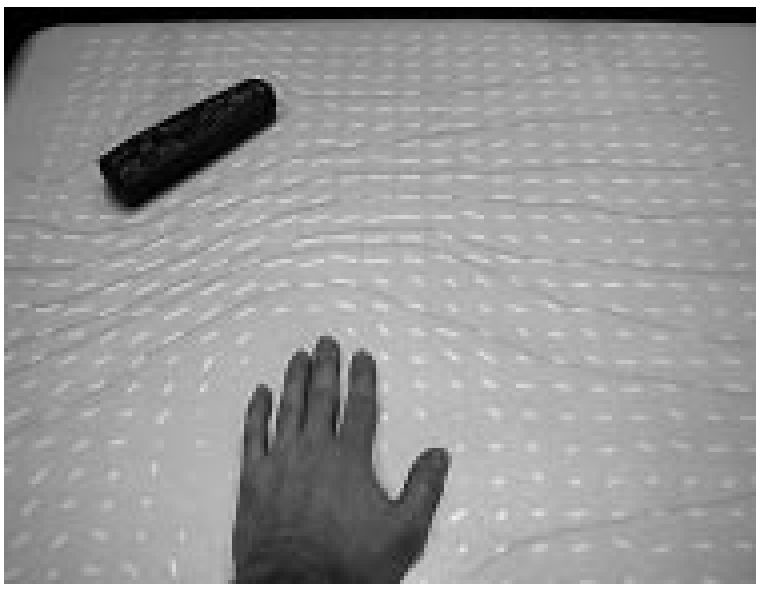
\includegraphics[width=0.45\textwidth]{figures/urp-fluid.jpg}
\caption{Flow visualization in Urp.}
\label{fig:urpa}
\end{figure}

For the wind simulation a variety of cellular automaton called a 'lattice gas' is employed to simulate pedestrian-level airflow. The hexagonal cells support up to six gas 'particles', one for each face. 
A small set of rules determines particle collisions at each timestep. Due to the small size of the grid it's not possible to represent arbitrary flow directions accurately. 
Engaging the airflow simulation can be accomplished by placing the wind-tool, a kind of inverse weather vane, anywhere on the table. Orienting the tool selects one of eight quantized directions. A regular array of white segments is displayed, whose direction and length show the direction and length of the wind at that position as can be seen in Figure \ref{fig:urpa}. 

The anemometer-object, an arrow-shaped tool, samples and numerically displays the flow magnitude at the precise position of the tool's tip.

The casting of shadows can be influenced by a clock who determines the time of the day. The transition in time values is interpolated using cubic splines. An example of such shadows can be seen in Figure \ref{fig:urp2}.

\textit{Urp} also provides a distance-tool, shaped like a pencil but with the image of a ruler stretching between the pencil tip and the eraser, that can be used to connect together selected structures. 

Traffic also can be simulated by placing \textit{voodoo}-tagged strips in the environment, engaging a traffic simulation. Crossing two strips generates an intersection. 

Touching a building with a special transparent wand causes the facade to become glass and solar reflections are generated. Using the other end of the wand, the facade can be transformed back into brick. 

A mechanism for 'previewing' a configuration of buildings from various points of views is also possible, since the model buildings are already resident in the system. They can be rendered with simple shading techniques. For this purpose a simple camera can be driven about the workspace and a real-time rendering of the current arrangement as viewed from pedestrian height becomes visible. 

\begin{figure}
\centering
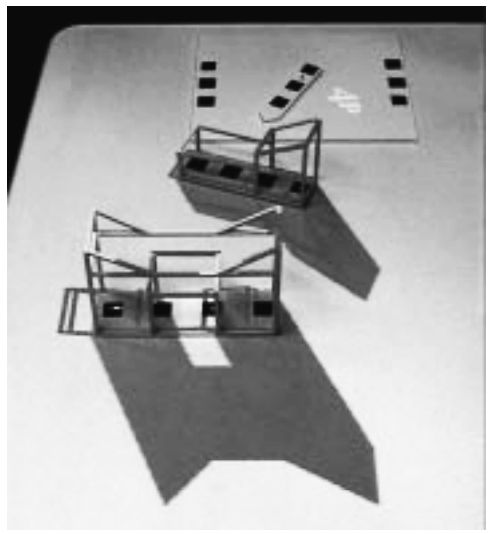
\includegraphics[width=0.45\textwidth]{figures/urp-shadow.jpg}
\caption{Shawods in Urp.}
\label{fig:urp2}
\end{figure}





\section{Including social aspects}

Hornecker and Buur \cite{hornecker06} extend the thought of tangible user interfaces further to 'tangible interactions'. They introduce a framework that focuses on the interweaving of the material/physical and the social, laying the ground for collaboration-sensitive tangible interaction design. It relies on tangibility and full-body interaction and gives computational resources and data material form, embedding computing in the everyday environment, digitally augmenting physical space and supporting intuitive use. 

"Designing tangible interfaces requires not only designing the digital but also the physical, and their interrelationships within hybrid ensembles, as well as designing new types of interaction that can be characterized as full-body, haptic, and spatial" \cite{hornecker06}.
Interfaces which previously wouldn't have been considered as such are turning into such and computing is increasingly embedded in physical environments.

They distinguished three different views on tangible interfaces:
\begin{itemize}
\item Data-centered view: Here 'tangible interfaces' are understood as utilizing physical representation and manipulation of digital data, offering interactive couplings of physical artifacts with "computationally mediated digital information" \cite{Holmquist04}.
\item Expressive-Movement-centered view: Aiming to design interaction itself by emphasizing bodily interaction with objects, exploiting the "sensory richness and action potential of physical objects" so that "meaning is created in the interaction" \cite{Djajadiningrat02}.
\item Space-centered view: 'Interactive spaces' as "Interactive systems, physically embedded within real spaces, offer opportunities for interacting with tangible devices" and so "trigger display of digital content or reactive behaviours" The body is used as interaction device and display \cite{Ciolfi04}.
\end{itemize}

Tangible interaction encompasses a broad range of systems and interfaces, building upon and synthesizing these views. These share the following characteristics: tangibility and materiality, physical embodiment of data, embodied interaction and bodily movement as an essential part of interaction, and embeddedness in real space, designing the interaction itself and exploiting the richness of bodily movement.

Their framework is structured around four interrelated themes \cite{hornecker06}:
\begin{itemize}
\item Tangible Manipulation:  material representations with distinct tactile qualities which are physically manipulated.
\item Spatial Interaction: tangible interaction is embedded in real space and therefore occurs by movement in space.
\item Embodied Facilitation: how the configuration of material objects and space affects and directs group behaviour.
\item Expressive Representation: material and digital representations employed by tangible interaction systems, their expressiveness and legibility.
\end{itemize}

\begin{figure}
\centering
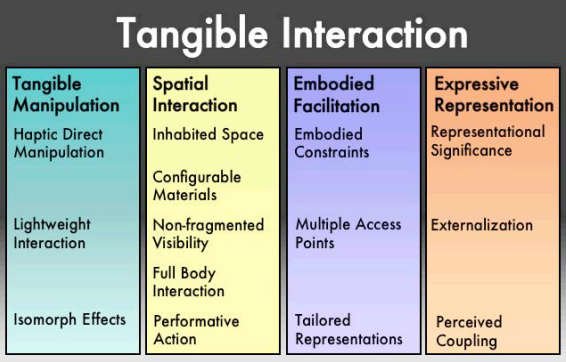
\includegraphics[width=0.45\textwidth]{figures/tangibleInteraction.png}
\caption{Tangible Interaction}
\label{fig:tangibleInteraction}
\end{figure}

Figure \ref{fig:tangibleInteraction} shows the design spaces of tangible interaction from specific on the left to the more general on the right. 

% Design and Hardware